\documentclass{midl}

\usepackage{booktabs}
\usepackage{xcolor}
\usepackage{siunitx}
\sisetup{detect-weight=true}

\jmlrvolume{-- Under Review}
\jmlryear{2027}
\jmlrworkshop{Validation Studies -- MIDL 2027 submission}
\editors{Under Review for MIDL 2027}

\newcommand{\pending}[1]{\textcolor{red}{[PENDING: #1]}}
\newcommand{\lam}{\lambda_{\mathrm{adv}}}
\newcommand{\xdomHalf}{0.270\,$\pm$\,0.034}
\newcommand{\xdomOne}{0.261\,$\pm$\,0.016}
\newcommand{\xdomFour}{0.276\,$\pm$\,0.025}
\newcommand{\xdomEight}{0.269\,$\pm$\,0.023}
\newcommand{\xdomEffb}{0.298\,$\pm$\,0.010}
\newcommand{\nAK}{202}
\newcommand{\nSCC}{66}
\newcommand{\nMEL}{9}
\newcommand{\repolink}{\url{https://github.com/TranDucVinh-20225538/CSG-SKin}}

\title[OOD Detection Inverts Under Gradient Reversal]{Out-of-Distribution Detection
Inverts Under Domain-Adversarial Training}

% TODO replace with the real author block before submission
\midlauthor{\Name{Author Name} \Email{author@example.edu}\\
 \addr Affiliation}

\begin{document}
\maketitle

\begin{abstract}
\noindent\textbf{Background.} Domain-adversarial invariance training is widely
recommended for removing acquisition shortcuts from medical imaging models. Its effect
on the out-of-distribution (OOD) monitoring such models rely on at deployment has not
been measured.

\noindent\textbf{Methods.} We swept the adversarial weight $\lam$ over seven values,
three to five seeds each (27 runs), on ISIC~2019 and PAD-UFES-20 with everything else
fixed, measuring domain leakage, in-distribution accuracy and calibration,
out-of-domain calibration, OOD detection with five scoring rules and zero-shot
cross-domain accuracy on a patient-level held-out partition. We repeated the sweep with
single-encoder adversarial training and four non-adversarial invariance objectives,
under a lesion-disjoint ISIC split, and on Fitzpatrick17k, never seen by the adversary.

\noindent\textbf{Results.} At the smallest non-zero weight OOD detection fell from
AUROC $0.843$ to $0.509$; by $\lam = 2$ it had \textbf{inverted below chance to
$0.427$} ($95\%$ CI $[0.414, 0.439]$) on the held-out PAD partition, with all five
seeds below $0.5$, ranking images from an unseen clinic as more in-distribution than
its own test data. All five rules
collapsed together and the inversion held on Fitzpatrick17k ($0.764 \to 0.391$). It was
invisible to routine monitoring: leakage fell to near its floor
($0.915 \to 0.571$, floor $0.5$), in-distribution accuracy ($0.692 \to 0.707$) and
calibration did not degrade, and the lesion-disjoint replication reproduced every
result ($0.808 \to 0.403$). Meanwhile out-of-domain calibration error tripled
($0.247 \to 0.746$) and actinic keratosis recall fell $0.245 \to 0.016$. After six
explanations were refuted, a mechanism satisfied three pre-registered criteria:
invariance is obtained by displacing out-of-domain images into the majority class's
region, their nearest-centroid share rising $0.332 \to 0.601$ while the
in-distribution share stays flat.

\noindent\textbf{Conclusions.} Across imaging modality, adversarial training does not
merely weaken OOD monitoring but reverses it, by the one move that defeats a
density-based novelty score, while every routinely monitored metric improves. Between
two hospitals sharing a modality the collapse persists and the reversal does not. OOD
detection and out-of-domain calibration should be reported as a function of achieved
invariance.
\end{abstract}

\begin{keywords}
domain-adversarial training; out-of-distribution detection; calibration; distribution shift; skin lesion classification; model monitoring
\end{keywords}



% ------------------------------------------------------------
\section{Introduction}

Deep models for skin lesion classification are known to exploit acquisition artefacts
rather than pathology: ruler marks, ink annotations, imaging hardware and site identity
all correlate with diagnosis in public benchmarks
\cite{winkler2019,bissoto2020,daneshjou2022}. The standard remedy is to make the
representation invariant to the acquisition domain, most often through
domain-adversarial training with a gradient reversal layer
\cite{ganin2016,bousmalis2016}, and its stated purpose is safe deployment across sites.
Deployment across sites also relies on a second mechanism: out-of-distribution
monitoring, by which a system flags inputs unlike its training data so a human reviews
them rather than the model acting alone. This paper asks what invariance training does
to that mechanism.

It reverses it. Sweeping the adversarial weight in a controlled setting, we find that
out-of-distribution detection does not merely weaken as domain information is removed
--- it passes through chance and inverts. At the weights that achieve invariance, a
model asked which inputs are unlike its training data answers with its own test split
and ranks images from a clinic it has never seen as the more routine of the two. AUROC
falls from $0.843$ to $0.427$, with a $95\%$ confidence interval of $[0.414, 0.439]$
lying entirely below chance, across every scoring rule we tried.

Degradation would be unsurprising: a representation stripped of domain information
should be worse at recognising a domain, and chance is what that argument predicts.
Inversion is not, and accounting for it took six refuted explanations and a failed
pre-registered synthetic reproduction before a mechanism held --- invariance is
obtained by displacing out-of-domain images into the region the majority class
occupies, which a density-based novelty score reads as familiarity.

What makes the reversal consequential rather than merely odd is that nothing in a
standard evaluation reveals it. Over the same range the model becomes more confident on
unseen-domain images than on its own held-out data and its predictions collapse toward
the benign majority class, while in-distribution accuracy does not fall,
in-distribution calibration does not change, and the domain leakage probe --- the very
metric the technique is adopted to improve --- improves exactly as intended. The
technique disables the cross-site safety machinery while every monitored number moves
in the direction its user is hoping for.

\paragraph{Contributions.}
\begin{enumerate}
\item A controlled intervention: a seven-point sweep of the adversarial weight,
27 training runs with everything else held fixed, isolating invariance pressure
from architectural and data confounds.
\item The inversion: OOD detection passes through chance and reverses, as a
cliff rather than a trade-off curve, across five scoring rules, on a third
dataset the adversary never saw, and robustly to shrinkage estimation and tail
truncation.
\item The invisibility: in-distribution accuracy, in-distribution calibration
and the domain leakage probe all fail to reveal it, under both an image-level and
a lesion-disjoint ISIC split at five seeds, and the leakage probe does not
mediate it, so it cannot serve as a proxy either.
\item Scope: the failure reproduces in plain single-encoder adversarial
training, so it is not an artefact of the factorized architecture; and it does
not appear under moment-matching objectives that reduce leakage along the same
axis, so it belongs to adversarial optimisation rather than to invariance.
\item A mechanism with predictive content, satisfying three pre-registered criteria
and replicating on a second representation, after six alternative accounts and a
pre-registered synthetic reproduction were tested and refuted.
\item A reporting protocol that makes the failure visible at near-zero cost.
\end{enumerate}

% ------------------------------------------------------------
\section{Related work}

\paragraph{Shortcut learning in dermatology.}
Ink markings shift melanoma predictions \cite{winkler2019}, classifiers keep
competitive ISIC accuracy with the lesion masked out \cite{bissoto2020}, and
performance degrades on darker skin tones \cite{daneshjou2022}. These motivate
invariance-based remedies.

\paragraph{Invariant representation learning.}
Domain-adversarial training \cite{ganin2016} and domain separation networks
\cite{bousmalis2016} remove domain information by adversarial or orthogonality
constraints. \textbf{The architecture used here is equivalent to a domain separation
network and is not a contribution of this paper}; it is a vehicle for the intervention.

\paragraph{Covariate shift versus semantic novelty.}
Full-spectrum OOD detection \cite{yang2023} argues the literature conflates two
shifts, and proposes a taxonomy --- training ID, \emph{covariate-shifted ID}, near-OOD
and far-OOD --- in which covariate-shifted in-distribution samples should be tolerated
rather than flagged, since rejecting them contradicts generalization; OpenOOD v1.5
\cite{zhang2023} adopts the same setting at ImageNet scale. Our contrast falls in the
covariate-shifted-ID cell, so a reader of \cite{yang2023} might regard a model that
accepts these images as behaving correctly. Section~\ref{sec:tolerance} argues
tolerance is safe only with generalization, and here it is not.

\paragraph{Calibration under adaptation, and the reverse direction.}
Calibration degrades under shift for ordinary training \cite{ovadia2019}, and domain
adaptation methods specifically \emph{trade} calibration for accuracy on the target
domain, for which a post-hoc correction exists \cite{wang2020}. \textbf{The calibration
degradation in Section~\ref{sec:confidently} is therefore not a new phenomenon.} New
here are its dose-dependence on the adversarial weight, its invisibility to
in-distribution calibration, and --- separately from calibration --- the collapse and
inversion of OOD detection, which a confidence correction does not address. In the
forward direction, enforcing multi-domain calibration yields invariance and provable
freedom from certain spurious correlations \cite{wald2021}; we find the reverse
implication does not hold (Section~\ref{sec:confidently}).

\section{Materials and methods}

\subsection{Data}

\textbf{ISIC 2019} \cite{isic2019}: 25{,}331 dermoscopic images, eight
diagnostic classes (MEL, NV, BCC, AK, BKL, DF, VASC, SCC), CC~BY-NC~4.0.
\textbf{PAD-UFES-20} \cite{pacheco2020}: 2{,}298 smartphone clinical
photographs, six classes mapping into the same label space (DF and VASC
absent), CC~BY~4.0. \textbf{Fitzpatrick17k} \cite{groh2021}: 3{,}887 of
16{,}577 images obtained; annotations CC~BY-NC-SA~3.0, images web-scraped
under mixed copyright, used for evaluation only and not redistributed.

Images were cropped to a soft lesion-centred bounding box via Otsu
thresholding on the deviation from the border median, expanded by a 0.30
margin with a 0.70 minimum crop ratio, and resized to $224\times224$.

\subsection{Splits and the PAD held-out set}

ISIC was split $60/20/20$ into train/validation/test, stratified by label
(\texttt{random\_state}~$=42$).

\textbf{PAD appears in training and would otherwise also be the OOD set.}
The classification loss never sees PAD labels (\texttt{ignore\_index}$=-1$),
but PAD images enter the context and adversarial branches. To remove the
resulting circularity we partitioned PAD \emph{at patient level} into
\texttt{pad\_adv} (1{,}582 images, 961 patients), visible to those branches
during training, and \texttt{pad\_heldout} (716 images, 412 patients), never
seen in any form. No patient and no lesion appears in both. \textbf{All OOD
and cross-domain numbers reported in the main text use
\texttt{pad\_heldout}.} An earlier draft of this work reported $0.413$ at $\lam = 2$;
that value was scored on \texttt{pad\_full}, which includes the $1{,}582$ images the
adversarial branch saw during training. Fitzpatrick17k provides a second never-adversarial
domain.

\subsection{Architecture and objective}

A dual-encoder model with EfficientNet-B3 backbones produces a lesion latent
$z_{\ell} \in \mathbb{R}^{16}$ (batch-normalised, denoted
$z_{\ell}^{\mathrm{norm}}$) and a context latent $z_{c} \in \mathbb{R}^{64}$.
Diagnosis uses $z_{\ell}^{\mathrm{norm}}$ only, through a linear head. The
objective is
\begin{equation}
\mathcal{L} = \mathcal{L}_{\mathrm{cls}}
+ \lambda_{\mathrm{ctx}}\mathcal{L}_{\mathrm{ctx}}
+ \lam\,\mathcal{L}_{\mathrm{adv}}
+ \lambda_{\mathrm{orth}}\mathcal{L}_{\mathrm{orth}},
\end{equation}
with $\mathcal{L}_{\mathrm{cls}}$ on ISIC only, $\mathcal{L}_{\mathrm{ctx}}$ a
domain cross-entropy on $z_c$, $\mathcal{L}_{\mathrm{adv}}$ a domain
cross-entropy on $z_{\ell}^{\mathrm{norm}}$ behind a gradient reversal layer,
and $\mathcal{L}_{\mathrm{orth}}$ a squared-cosine penalty between the two
latents ($\lambda_{\mathrm{orth}} = 1$ throughout).

AdamW, base learning rate $10^{-4}$, adversary learning rate multiplier $30$,
classifier multiplier $0.2$, 40 epochs, batches balanced across domains,
checkpoint selected on validation accuracy.

\subsection{The intervention}

$\lam \in \{0,\,0.25,\,0.5,\,1,\,2,\,4,\,8\}$; five seeds at
$\lam \in \{0, 2, 8\}$ and three at the interior points, for 27 runs.
Everything else is held fixed, so $\lam$ is the only manipulated variable.

\subsection{Measurements}

\paragraph{Domain leakage.} Logistic probe on frozen features predicting the
source dataset, reported as \textbf{balanced accuracy, whose chance floor is
$0.5$ for this two-domain problem}. Earlier work on this dataset pair reports
plain accuracy against a majority floor of $0.688$; the two scales must not be
compared to each other. Both are stated where relevant.

\paragraph{OOD detection.} Maximum softmax probability \cite{hendrycks2017}, free
energy \cite{liu2020}, maximum cosine to a class centroid, class-conditional
Mahalanobis with shared covariance \cite{lee2018}, and $k$-NN distance
\cite{sun2022} ($k \in \{10,50,200\}$), all fit on the ISIC training split alone.
\textbf{These five rules are not independent evidence}: the classifier is a linear map
from $z_{\ell}^{\mathrm{norm}}$, so all five are functions of the same
$16$-dimensional vector. Independent evidence comes from the pre-projection backbone
(Section~\ref{sec:nonmediation}).

\paragraph{Calibration.} Expected calibration error, 15 bins, on ISIC test and on
\texttt{pad\_heldout} restricted to the six shared classes. \textbf{Out-of-domain ECE
here is arithmetically close to mean confidence minus accuracy}, so the confidence,
accuracy and ECE results in Section~\ref{sec:confidently} are three views of one
phenomenon rather than three findings.

\paragraph{Uncertainty.} Intervals on AUROC come from a stratified bootstrap,
2{,}000 resamples, percentile method, fixed in a pre-registration before the values
were computed. Each draw resamples \textbf{patients} from \texttt{pad\_heldout} and,
independently, images from the ISIC test split, because AUROC depends on both score
distributions and resampling one side understates the interval; within a draw the same
resampled sets serve every seed. We report the interval on the five-seed mean and the
number of seeds whose own interval clears $0.5$. Fitzpatrick17k carries no patient
identifiers, so its bootstrap is over images and its interval is likely
anti-conservative.

\paragraph{Cross-domain diagnosis.} Zero-shot on \texttt{pad\_heldout} over the six
shared classes; PAD labels were never used for $\mathcal{L}_{\mathrm{cls}}$.

% ------------------------------------------------------------

\section{Results}

\subsection{The intervention}

Table~\ref{tab:dial} reports every measurement as a function of $\lam$, the only
manipulated variable. Figure~\ref{fig:dial} shows the four quantities that matter most
on a shared axis.

Read across a single row and nothing is wrong. Read down the columns and two of them
improve while two collapse.

\begin{table}[t]
\centering
\small
\caption{The intervention. Mean $\pm$ s.d.\ across seeds. Leakage is balanced accuracy
(chance $0.5$); cross-domain accuracy is balanced over the six classes shared with
PAD-UFES (chance $0.167$). Arrows mark the direction a practitioner would call
favourable. The $\lam = 0.25$ row previously reported three-seed means for
leakage, in-distribution accuracy and Fitzpatrick AUROC while declaring $n = 5$;
those three are corrected here, and the $\lam = 0.25$ and $\lam = 1$ rows are now
final at five seeds. $^{\dagger}$ marks the one cell still at three seeds, the
$\lam = 1$ out-of-domain ECE.}
\label{tab:dial}
\resizebox{\textwidth}{!}{%
\begin{tabular}{lcccccccc}
\toprule
$\lam$ & $n$ & Leakage $\downarrow$ & ID bal.\ acc $\uparrow$ & ID ECE
& OOD ECE & OOD AUROC & Fitz.\ AUROC & X-dom bal.\ acc \\
\midrule
0    & 5 & 0.915\,$\pm$\,0.021 & 0.692 & 0.107 & 0.247 & \textbf{0.843\,$\pm$\,0.023} & 0.764\,$\pm$\,0.038 & 0.291\,$\pm$\,0.016 \\
0.25 & 5 & 0.571 & 0.692 & 0.101 & 0.684 & \textbf{0.509} & 0.460 & 0.291\,$\pm$\,0.020 \\
0.5  & 3 & 0.555\,$\pm$\,0.029 & 0.701 & 0.096 & 0.724 & 0.465\,$\pm$\,0.015 & 0.449\,$\pm$\,0.025 & \xdomHalf \\
1    & 5 & 0.591 & 0.695 & 0.097 & 0.733$^{\dagger}$ & 0.457 & 0.414 & \xdomOne \\
2    & 5 & 0.584\,$\pm$\,0.027 & 0.707 & 0.099 & 0.746 & \textbf{0.427\,$\pm$\,0.025} & 0.391\,$\pm$\,0.068 & 0.249\,$\pm$\,0.030 \\
4    & 3 & 0.548\,$\pm$\,0.035 & 0.686 & 0.100 & 0.726 & 0.455\,$\pm$\,0.039 & 0.431\,$\pm$\,0.036 & \xdomFour \\
8    & 5 & 0.625\,$\pm$\,0.045 & 0.679 & 0.099 & 0.713 & 0.494\,$\pm$\,0.027 & 0.474\,$\pm$\,0.060 & \xdomEight \\
\midrule
\multicolumn{2}{l}{EffNet-B3 control} & 0.802 & 0.683 & 0.096 & --- & 0.726\,$\pm$\,0.021 & 0.649 & \xdomEffb \\
\multicolumn{2}{l}{ResNet-50 baseline} & 0.979 & 0.655 & 0.101 & --- & 0.868\,$\pm$\,0.019 & 0.994 & 0.391 \\
\bottomrule
\end{tabular}}
\end{table}

\begin{figure}[t]
\centering
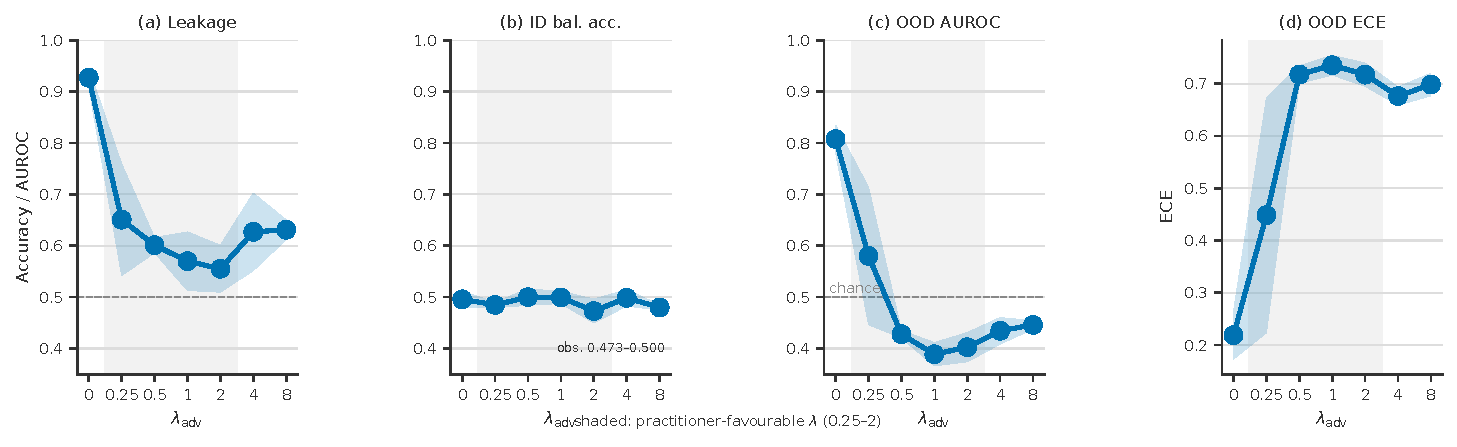
\includegraphics[width=\textwidth]{../../results/paperB/figures/fig1_intervention.pdf}
\caption{\textbf{The intervention, four views, one axis.} Leakage falls to its chance
floor and in-distribution balanced accuracy does not degrade --- both favourable. Over
the same range OOD AUROC collapses through chance and inverts, and out-of-domain
calibration error triples. A developer monitoring the first two panels would see
nothing wrong.}
\label{fig:dial}
\end{figure}

\subsection{Invariance is achieved, and in-distribution metrics do not warn}

Domain leakage falls from $0.915$ to $0.571$ between $\lam = 0$ and $\lam = 0.25$,
against a chance floor of $0.5$. By the smallest non-zero weight tested, the lesion
representation is very nearly uninformative about the acquisition source: the intended
effect of the method, obtained essentially in full.

It is obtained without an in-distribution cost. Balanced accuracy on the ISIC test
split moves from $0.692$ to $0.707$ over the useful range --- we claim no improvement,
the difference being small relative to seed variance --- and in-distribution expected
calibration error is flat at $\approx 0.10$ at every $\lam$. A practitioner tracking
accuracy, in-distribution calibration and the leakage probe would conclude that the
method had worked exactly as advertised.

\subsection{Out-of-distribution detection collapses, and inverts}

Over the same interval, Mahalanobis AUROC against the held-out PAD partition falls
from $0.843$ to $0.509$ and reaches $0.427$ at $\lam = 2$. Two features matter more
than the size of that drop.

\paragraph{The fall to chance is a cliff; the inversion develops after it.} Almost
the whole descent happens in one step, $0.843$ to $0.509$ between $\lam = 0$ and
$\lam = 0.25$. The sub-chance
region is reached only at $\lam \geq 0.5$, after which the value moves between
$0.427$ and $0.494$ with no ordering a practitioner could tune against. So detection
collapses to chance at the smallest non-zero weight tested and inverts under further
pressure; there is no operating point at which invariance has been obtained and
detection survives.

\paragraph{It goes below chance.} At $\lam = 2$ the detector ranks images from a
clinic the model has never seen as \emph{more} in-distribution than its own test
split. A patient-clustered bootstrap puts the $95\%$ interval at $[0.414, 0.439]$ with
all five seeds' individual intervals below $0.5$; the same holds for $k$-NN ($0.440$,
$[0.429, 0.452]$, $5/5$) and, one seed short, cosine ($0.453$, $[0.441, 0.464]$,
$4/5$). It is not a tail artefact: removing the pooled $90$th, $95$th or $99$th
percentile leaves AUROC at $0.412$, $0.416$ and $0.424$ against $0.427$ for the full
set, and the medians themselves invert (ISIC $13.8$ versus \texttt{pad\_heldout}
$10.0$).

All five rules move together --- MSP $0.970 \to 0.437$, energy $0.983 \to 0.441$,
cosine $0.901 \to 0.435$, $k$-NN $0.941 \to 0.424$, stable across
$k \in \{10, 50, 200\}$ --- but as noted in the methods they are five views of one
$16$-dimensional representation; the independent replications are the backbone
(Section~\ref{sec:nonmediation}) and the single-encoder model
(Section~\ref{sec:arch}).

Three artefact explanations fail. \emph{Covariance estimation:} Ledoit--Wolf
shrinkage leaves $\lam = 2$ at $0.427$, and across float32 and float64, with and
without shrinkage, at one, four and eight BLAS threads, the largest AUROC deviation is
$9.4 \times 10^{-4}$; effective dimensionality barely moves (participation ratio
$4.879 \to 4.500$ while leakage falls $0.914 \to 0.553$ in the same three runs).
\emph{An over-strong adversary:} the adversary runs at $30\times$ the base learning
rate, and retraining at $10\times$ and $100\times$ keeps the inversion ---
$0.418 \pm 0.011$ at $10\times$ with all three seeds below $0.5$, against
$0.432 \pm 0.024$ at $30\times$ and $0.482 \pm 0.020$ at $100\times$ (one seed at
$0.503$) --- so weakening it tenfold deepens the inversion rather than removing it.
\emph{The adversary's own domain:} on Fitzpatrick17k, absent from every training
branch, AUROC falls $0.764 \to 0.391$ ($95\%$ CI $[0.386, 0.396]$, five of five seeds
below $0.5$; bootstrapped over images, so likely anti-conservative). For context a
ResNet-50 baseline reaches $0.994$ on those images and the EfficientNet-B3
single-encoder control $0.649$; the controlled comparison is the $\lam = 0$ row, which
differs from $\lam = 2$ only in the adversarial weight.

\subsection{The model becomes confidently wrong on unseen domains}
\label{sec:confidently}

Confidence rises as competence falls. At $\lam = 0$ mean maximum-softmax confidence is
$0.915$ on ISIC test and $0.489$ on \texttt{pad\_heldout}; by $\lam = 2$ the ordering
has inverted, $0.930$ on a clinic the model has never seen against $0.910$ on its own
test set, while cross-domain balanced accuracy never improves at any $\lam$
($0.249$--$0.291$ against a floor of $0.167$) and predictions collapse toward the
benign majority class, with \textbf{actinic keratosis recall falling
$0.245 \to 0.016$}. Out-of-domain calibration error triples, $0.247 \to 0.746$, while
in-distribution ECE stays flat at $\approx 0.10$, so no in-distribution measurement
reveals it. That adapted models are miscalibrated on the target domain is known
\cite{wang2020}; what the sweep adds is the dose-dependence and the invisibility, and
we stress that confidence, accuracy and calibration here are three views of one
phenomenon rather than three results (Appendix~\ref{app:confident}).

\subsection{Leakage does not mediate the collapse}
\label{sec:nonmediation}

The natural hypothesis is that removing domain information is what breaks detection.
Four results rule it out, the last of them outside dermatology.

First, leakage \textbf{falls to within $0.07$ of its chance floor by
$\lam = 0.25$} ($0.571$ against a floor of $0.5$) and goes no lower at any larger
weight while AUROC continues to fall from $0.513$ to $0.427$ as $\lam$ rises
further. The damage continues after invariance is complete.

Second, at the pre-projection backbone, leakage is essentially flat across the whole
sweep ($0.982 \to 0.941$) while backbone Mahalanobis AUROC falls $0.749 \to 0.475$.
Domain information remains linearly decodable there, and detection collapses anyway.
Because the backbone is a different representation from the $16$-dimensional latent,
this is the independent replication that the five-detector agreement does not provide.

Third, and most directly, two training objectives traverse the same leakage range with
opposite consequences (Section~\ref{sec:adversarial}). Leakage alone therefore does not
determine the outcome.

Fourth, in histopathology the two quantities come apart almost completely. In a
two-hospital Camelyon17 setting (three seeds, hospital-disjoint slides held out
for detection), raising $\lam$ from $0$ to $1$ moves all five detectors by
$0.12$ to $0.22$ --- Mahalanobis $0.651 \to 0.534$, cosine $0.785 \to 0.589$,
$k$-NN $0.794 \to 0.648$, MSP $0.798 \to 0.589$, free energy
$0.794 \to 0.575$ --- while the hospital probe moves by $0.007$
($0.959 \pm 0.007 \to 0.952 \pm 0.001$), which is inside its own seed spread at
$\lam = 0$, and in-distribution accuracy is unchanged at $0.995$. The adversary
reached chance here (final cross-entropy $0.692$ against $\ln 2 = 0.693$), so
the optimisation pressure was applied; the encoder simply did not become
invariant under it. Detection degraded regardless. \textbf{This is the clearest
dissociation we obtained: the outcome moved roughly twenty-five times as far as
the supposed mediator.}

Two qualifications. The detectors fall but remain above chance ($0.53$--$0.65$),
so this is degradation, not the collapse to chance seen in dermatology, and
nothing here bears on the inversion. And these runs come from an experiment that
failed its own pre-registered gate --- we had required the probe to fall by at
least $0.10$ before treating the setting as a test of invariance, and it fell by
$0.007$. That gate failure is precisely what makes the runs informative here:
they are a case where invariance was \emph{not} obtained and detection degraded
anyway. We report them for this claim only, and the pre-registered verdict on
the original question stands as negative (Section~\ref{sec:limitations}).

We accordingly report leakage as a measured quantity and never as the explanatory
variable, and plot all results against $\lam$ rather than against leakage.




\subsection{The failure is specific to gradient reversal}
\label{sec:adversarial}

Adversarial training is one route to invariance among several. Table~\ref{tab:obj}
sweeps four alternatives on the single-encoder backbone: deep CORAL
\cite{sun2016coral}, maximum mean discrepancy \cite{long2015}, invariant risk
minimisation \cite{arjovsky2019} and group distributionally robust optimisation
\cite{sagawa2020}.


Only MMD moves leakage appreciably, and it does so at a price gradient reversal never
pays. Escalating the MMD weight from $1$ to $10{,}000$ buys $0.13$ of leakage
($0.967 \to 0.836$, floor $0.5$) at a cost of $0.44$ of in-distribution balanced
accuracy ($0.779 \to 0.337$), and leaves every detector well above chance
(Mahalanobis $0.665$, $k$-NN $0.738$, energy $0.694$ at the highest weight). IRM
reaches the extreme of the same pattern: at weight $100$ its balanced accuracy collapses
to $0.167$ while leakage remains at $0.950$. CORAL does not induce invariance at all;
at weight $100$ it makes the representation \emph{more} domain-separable
(leakage $0.998$). GroupDRO leaves leakage unmoved at every weight tested.

The contrast is cleanest when task health is held constant rather than leakage, since
MMD only reaches comparable leakage by destroying the classifier:

\begin{quote}
Gradient reversal reduces leakage $0.970 \to 0.763$ \textbf{at no cost in accuracy}
($0.845 \to 0.845$) and collapses all five detectors to chance. MMD reduces leakage
$0.967 \to 0.900$ at a similarly negligible cost ($0.779 \to 0.730$) and collapses
nothing (Mahalanobis $0.813 \to 0.716$). To go further, MMD must destroy the task.
\emph{Out-of-domain set for the MMD figures: \pending{R4}; the comparison is only
valid if both arms are scored on \texttt{pad\_heldout}.}
\end{quote}

The calibration signatures differ in the same direction. As MMD degrades, its
out-of-domain ECE \emph{falls} ($0.344 \to 0.142$): the model becomes less confident as
it becomes less accurate, which is the appropriate response. Under gradient reversal
out-of-domain ECE triples while accuracy falls. The two objectives move leakage the same
way and fail in opposite manners --- one degrades honestly, the other is confidently
wrong.

We do not claim MMD would be safe at the invariance level gradient reversal reaches; it
never got there. What the data establish is that at the leakage levels MMD does reach,
it shows none of the failure, while gradient reversal at the same levels has already
collapsed.

\subsection{It is not specific to the factorized architecture}
\label{sec:arch}

All results above use a dual-encoder model. Repeating the sweep with plain
single-encoder domain-adversarial training --- one backbone, one linear classifier, a
gradient reversal layer and a domain head, with no context branch and no orthogonality
term --- reproduces the cliff: every detector collapses at $\lam = 0.25$ and by
$\lam = 4$ four of the five sit below chance, while in-distribution accuracy stays flat
(Appendix~\ref{app:single}, Table~\ref{tab:single}). \textbf{The invisibility, the
collapse and the inversion are therefore properties of domain-adversarial training
rather than of the factorized architecture.}

\paragraph{A second backbone leaves the question open.} Repeating the single-encoder
sweep with a ResNet-50 backbone did not settle whether the inversion is specific to
EfficientNet-B3, because comparable invariance was never reached. At
$\lam = 2$ the adversary never left chance --- best-epoch cross-entropy $0.686$ to
$0.688$ against a threshold of $0.673$ --- so those three runs are null experiments and
we draw no conclusion from them. At $\lam = 0.5$, where the adversary did learn
(best-epoch cross-entropy $0.41$ to $0.55$), leakage fell only from $0.965$ to $0.939$
against the $0.742$ that EfficientNet-B3 reaches on the same partition, so invariance
was not obtained and the backbone question is untested rather than answered in the
negative.

\textbf{On that run the detectors disagree, and we report all of them rather than
the one that suits each point.} Over the same $\lam = 0 \to 0.5$ step, $k$-NN falls
$0.962 \to 0.563$ and cosine $0.922 \to 0.543$, while Mahalanobis moves only to
$0.814$ and never approaches chance. Three detectors that move together on
EfficientNet-B3 separate here. We draw two things from this, and no more. Taking
the detectors that do move, the step is the sharpest non-mediation evidence in the
paper: the outcome shifts by $0.40$ while leakage, the supposed mediator, shifts by
$0.026$ (Section~\ref{sec:nonmediation}). Taking Mahalanobis, the headline detector
everywhere else in this paper, nothing happens. \textbf{The claim that all five
scoring rules collapse together therefore holds on EfficientNet-B3 and does not
hold here}, which is an additional reason the backbone question is open.

One difference is informative. The single-encoder model plateaus at leakage
$0.76$--$0.81$ and never reaches the $0.571$ the dual-encoder attains; more adversarial
pressure buys no further invariance. The dual-encoder has somewhere to put the
discarded information --- a domain probe on its context branch reads $>0.9999$ --- while
the single-encoder must destroy it. The architecture that achieves deeper invariance
also suffers the larger collapse ($0.427$ versus $0.509$ at $\lam = 2$), which is the
dose--response relationship seen from a second direction.

\subsection{The collapse generalises to a same-modality site shift; the inversion does not}
\label{sec:site}

Every result above contrasts dermoscopy with clinical photography, so the construct we
call domain is confounded with imaging modality. ISIC~2019 contains a contrast that is
not: its \texttt{lesion\_id} field records the contributing site, with $12{,}413$ images
from Hospital Cl\'inic Barcelona (\texttt{BCN}) and $10{,}015$ from the HAM10000
collection (\texttt{HAM}) --- two hospitals, two dermatoscopes, two patient
populations, one modality. The two sites are separable from frozen ERM features at
balanced accuracy $0.962 \pm 0.007$, comparable to the $0.970$ that
ISIC$\leftrightarrow$PAD reaches, and not for trivial reasons: masking the
dermatoscope vignette costs only $0.019$, hand-crafted colour statistics reach
$0.901$ against a $0.876$ ceiling on the original pair, and a label-only probe
reaches $0.668$ (Appendix~\ref{app:site}).

\textbf{The collapse reproduces.} With \texttt{BCN} in distribution and a
lesion-disjoint $30\%$ \texttt{HAM} partition held out, leakage falls
$0.963 \pm 0.006 \to 0.821 \pm 0.030$ at $\lam = 0.25$ and the detectors with
headroom fall through chance: $k$-NN $0.658 \pm 0.041 \to 0.486 \pm 0.009$, cosine
$0.576 \pm 0.040 \to 0.477 \pm 0.006$ (3 seeds). Unlike the two multi-domain settings
in the limitations, the manipulation took.

\textbf{The inversion does not.} Reversing the roles restores detector headroom ---
Mahalanobis reads $0.846 \pm 0.003$ at $\lam = 0$, essentially the $0.843$ of the
dermatology sweep --- and adversarial training then reduces leakage from $0.95$ to
$0.77$ and drives Mahalanobis to $0.683 \pm 0.015$ at $\lam = 1$, where the
patient-clustered bootstrap gives $[0.666,\, 0.699]$ with all three seeds' intervals
entirely above $0.5$. Detection degrades substantially and stops above chance.

\textbf{Reading.} Baseline detectability is the same ($0.846$ versus $0.843$) and the
achieved invariance is the same as the single-encoder dermatology run ($0.77$ versus
$0.763$), yet the cross-modality contrast reaches $0.427$ while the same-modality one
stops at $0.683$. Neither a shortage of headroom nor a shortfall in achieved
invariance accounts for the gap, so we separate two claims the earlier sections report
together. The \emph{collapse} --- detection falling to chance as invariance is
obtained, invisibly to in-distribution metrics --- reproduces between two hospitals.
The \emph{inversion} does not: in every setting where we observe it the two domains
differ in imaging modality. Whether that reflects a threshold in the size of the shift,
something specific to modality gaps, or a property of these datasets, we cannot say.

\subsection{The pattern survives a lesion-disjoint split, but the invisibility
to accuracy does not}
\label{sec:lesionsplit}

This paper is about shortcut learning, and its main sweep uses an image-level
ISIC split in which $3{,}041$ of $5{,}067$ test images ($60.0\%$) share a
\texttt{lesion\_id} with training or validation. We therefore repeated
$\lam \in \{0, 2\}$ with the ISIC split grouped by \texttt{lesion\_id}, five
matched seeds, everything else fixed. Images with a null \texttt{lesion\_id}
($8.23\%$) each form their own group; no lesion crosses any partition.

Every pre-committed pattern check passes. Leakage still falls
($0.927 \pm 0.018 \to 0.555 \pm 0.046$), in-distribution ECE is unchanged at
$0.181$, out-of-domain ECE still rises ($0.219 \to 0.717$), all five detectors
still fall, and the inversion still holds on both out-of-domain sets:
Mahalanobis $0.808 \to 0.403$ on \texttt{pad\_heldout}, bootstrap CI
$[0.380, 0.425]$ with all five seeds individually below $0.5$, and
$0.717 \to 0.402$ on Fitzpatrick17k, CI $[0.390, 0.415]$.
In-distribution balanced accuracy does not degrade here either: it reads
$0.496 \pm 0.016$ at $\lam = 0$ against $0.473 \pm 0.023$ at $\lam = 2$, but the
paired per-seed difference is $-0.023$ with a CI of $[-0.063, +0.017]$, which
contains zero. We report it as a trend and claim nothing from it.

\textbf{What the honest split does change is the absolute level, and by far
more than $\lam$ ever does.} Removing the lesion overlap costs $0.20$ of
balanced accuracy at $\lam = 0$ ($0.692 \to 0.496$), consistent with the
companion analysis of lesion-level leakage in this dataset \cite{leakagepaper}.
The leakage this paper is
about is therefore worth roughly ten times the largest effect we attribute to
the adversarial weight, and the in-distribution accuracies in Table~\ref{tab:dial}
are optimistic by that amount. It does not disturb any comparison across $\lam$,
all of which are made under one split.

The difference between the two splits is not a change in class balance: the
lesion-level test set has the same class distribution to within one image in
every class, and reweighting it to the image-level mix leaves every detector
value identical to three decimal places.

\subsection{The inversion runs through the majority-class centroid}
\label{sec:mechanism}

Nevus is $50.8\%$ of the in-distribution set. We pre-registered three criteria for the
hypothesis that gradient reversal moves out-of-domain images into the nevus region of
the latent space, and all three hold.

\textbf{(i) Out-of-domain images migrate to the nevus cell.} The fraction of
\texttt{pad\_heldout} images whose nearest class centroid is nevus rises from $0.332$
at $\lam = 0$ to $0.601$ at $\lam = 2$ ($\Delta = 0.268$ against
$2\,\mathrm{SE} = 0.055$), while the same fraction for in-distribution images is flat
($0.528 \to 0.531$). It tracks the diagnostic shift: across all 27 runs the
correlation between this fraction and the number of \texttt{pad\_heldout} images
predicted nevus ($105 \to 424$ of $716$) is $\rho = 0.982$.

\textbf{(ii) The inversion is confined to those images.} Split by nearest centroid,
AUROC on the nevus-nearest subset falls $0.807 \to 0.282$ while the remainder stays
above chance throughout ($0.861 \to 0.644$).

\textbf{(iii) They move, and the reference does not.} Against a class-matched
reference --- in-distribution images that are themselves nevus --- the median squared
Mahalanobis distance from out-of-domain images to the nevus centroid falls from $49.8$
to $17.5$, while the reference distance is unchanged ($7.5 \to 7.4$).

The pattern replicates on the pre-projection backbone, a different representation of
$1536$ dimensions (nevus-nearest fraction $0.484 \to 0.603$, nevus-nearest AUROC
$0.726 \to 0.330$), so it is not a property of the $16$-dimensional projection.

\textbf{What the mechanism does not say.} Out-of-domain images never become more
typical than real nevi: the distance ratio stays above $1$ at every weight
($6.63 \to 2.37$). The inversion is a property of the \emph{pooled} AUROC, which
mixes classes. Pooled AUROC equals the class-share-weighted mean of the per-class
AUROCs, since AUROC averages over the in-distribution samples --- an identity, not a
result, which we use only to locate the effect. \textbf{The content is the two
per-class values: $0.559$ against nevus and $0.296$ weighted over the other five.}
Out-of-domain images are close to indistinguishable from nevi, whose centroid they are
drawn toward, and inverted against everything else; because the majority class is half
the data, the pooled score crosses chance. With all eight classes present the identity
holds to machine precision at every weight, both out-of-domain sets and both
in-distribution sets (largest residual $2.2 \times 10^{-16}$); restricted to the six
PAD-shared classes the discrepancy reaches $0.010$, the weight of the two omitted
classes. It also explains why per-class and pooled AUROC disagree at $\lam = 0$
(Section~\ref{sec:perclass}).

This accounts exactly for a result we had reported and could not previously explain.
Reweighting the in-distribution set to PAD's class mix --- $12.3\%$ nevus against
ISIC's $50.8\%$ --- \emph{strengthens} the inversion to $0.259 \pm 0.022$
(Table~\ref{tab:refuted}), because thinning nevus from the reference makes images
sitting in the nevus region look comparatively more typical. Reweighting changes only
the weights $w_c$; the model, every image's score and the out-of-domain set are
untouched, so no per-class AUROC moves, and evaluating $\sum_c w_c \mathrm{AUROC}_c$
under PAD's mix reproduces the measurement to $8 \times 10^{-7}$. A two-group
reduction does not, giving $0.306$, which is why the magnitude appeared not to follow
from the mechanism until the full form was used.

One consequence is worth stating with its scope. \textbf{For the pooled score, with
the model and out-of-domain set fixed, the inversion is deeper the \emph{less} the
in-distribution set is dominated by its majority class}: the two-group reduction
$0.559p + 0.296(1-p)$ for a nevus share $p$, with the non-nevus classes at ISIC
proportions, returns above chance only at $p = 0.776$. That is a statement about one
metric under one model, not a rule about deployments.

\subsection{What the phenomenon is not}


Table~\ref{tab:refuted} in the appendix lists six candidate accounts --- memorisation
of the adversarial images, class composition, domain specificity, dimensional collapse,
latent compression and tail asymmetry --- each tested against a prediction fixed before
its test, and each refuted, together with a pre-registered synthetic reproduction that
failed to reproduce the inversion. We report them because they are the reason the
account in Section~\ref{sec:mechanism} is credible: it is what survived after the
alternatives were eliminated, rather than the first story we tried.

\section{Discussion}

\paragraph{An inversion, not a degradation.}
The central result is not that out-of-distribution detection weakens under
adversarial invariance training but that the ordering reverses: at $\lam = 2$ a
model asked which images are unlike its training data answers with its own test
split. Degradation would be unsurprising --- a representation stripped of domain
information should be less able to recognise a domain --- and chance is what that
argument predicts, which is what a single-encoder model reaches at
$\lam = 0.25$ ($0.525$). Going \emph{past} chance is not predicted by it, and is
what Section~\ref{sec:mechanism} accounts for.

\paragraph{The deployment pathway.}
The results compose into one failure sequence. A model is trained with invariance
to acquisition domain, as recommended, and deployed at a new site, where it
increasingly predicts the benign majority class --- actinic keratosis recall
$0.245 \to 0.016$ --- with higher confidence than on its own test data. The
monitor that should flag those images does not merely fail to flag them; it ranks
them as more routine than familiar ones. Meanwhile the developer's evaluation
shows in-distribution accuracy holding, in-distribution calibration unchanged and
the leakage metric improved exactly as intended.

\paragraph{The failure belongs to gradient reversal, not to invariance.}
Reducing leakage is not sufficient to produce it. MMD reduces leakage along the
same axis and collapses nothing at the levels it reaches with the classifier
intact, where gradient reversal has already inverted. The two also fail in
opposite manners: pushed harder, MMD becomes less accurate \emph{and} less
confident and its out-of-domain calibration error falls, while under gradient
reversal accuracy falls as confidence rises and calibration error triples. One
degrades honestly, the other is confidently wrong. Two bounds follow. We cannot
rule out that MMD would behave the same way at the invariance level gradient
reversal reaches, because it never got there without destroying the task; and we
tested one adversarial formulation, so whether CDAN or adversarial discriminative
adaptation behaves like gradient reversal is not established here. The claim is
stated for gradient reversal, not for adversarial training in general.

\paragraph{The danger zone is where the method succeeds.}
Risk scales with \emph{achieved} invariance, not with the nominal weight or the
presence of an adversarial term. Where the adversary never learned, leakage stayed
at $0.94$ across four orders of magnitude of $\lam$ and the safety failure did not
appear either. A weak adversary produces neither debiasing nor harm --- so many
deployed configurations may be harmless, and a configuration's safety cannot be
read off its hyperparameters.

\paragraph{Tolerance without generalisation.}\label{sec:tolerance}
Full-spectrum OOD detection \cite{yang2023} prescribes that covariate-shifted
in-distribution inputs be accepted rather than flagged. Our models achieve that
prescription and are unsafe because of it: by $\lam = 2$ they accept out-of-domain
images more readily than their own test data while classifying them at $0.249$
balanced accuracy against a floor of $0.167$, with higher confidence than in
distribution. Acceptance and competence are separate properties, and current
protocols evaluate them separately or not at all. Any claim of tolerance to
covariate shift should carry cross-domain accuracy on the same inputs, since
tolerating inputs a model cannot classify is a failure mode rather than a success.

\paragraph{Two routes to invariance are not interchangeable.}
Wald et al.~\cite{wald2021} showed that enforcing multi-domain calibration
produces invariance. The converse fails: obtaining invariance adversarially
destroys out-of-domain calibration, driving ECE from $0.247$ to $0.746$. The
property one route builds on is the one the other removes. Where invariance is the
goal, calibration-based or moment-matching objectives may therefore be preferable,
because they reach it through constraints that leave the out-of-domain uncertainty
signal intact. Our MMD results are consistent with that, but we have not tested it
directly and offer it as a hypothesis rather than a finding.

\paragraph{Recommendation.}
Report OOD detection and out-of-domain calibration \textbf{as a function of achieved
invariance} rather than at a single operating point; report cross-domain accuracy
alongside any claim of tolerance to covariate shift; and state, when a separate
dataset serves as the OOD set, that this measures covariate shift rather than
semantic novelty. Practitioners tuning $\lam$ already train at several values, so
this changes what is reported rather than what is run. It converts an invisible
failure into a visible number.

\paragraph{Monitor outside the adversarial path.}
Since the collapse is a property of the representation that received adversarial
gradient, one mitigation is to score novelty on a representation that did not. A
frozen ImageNet ResNet-50 gives Mahalanobis AUROC $0.988$ on Fitzpatrick17k and
$0.833$ on \texttt{pad\_heldout}, against the trained model's $0.764$ and $0.843$ at
$\lam = 0$ and $0.391$ and $0.427$ at $\lam = 2$. It never inverts, but \textbf{we
had pre-registered $0.90$ in all four cells and \texttt{pad\_heldout} does not reach
it}, where the frozen encoder merely matches the untrained model rather than
improving on it. A partial mitigation, not a fix; retreating to an earlier layer of
the \emph{same} encoder does not work at all (Section~\ref{sec:nonmediation}).

\paragraph{The inversion is deepened, not created, in the minority classes.}
\label{sec:perclass}
Per-class AUROC, which unlike the pooled value does not depend on the ID class mix,
is $0.14$--$0.39$ on \texttt{pad\_heldout} and $0.10$--$0.34$ on Fitzpatrick17k at
$\lam = 2$ for every non-nevus class. Two are already at or below chance beforehand: on
\texttt{pad\_heldout} at $\lam = 0$, actinic keratosis is $0.499$ and squamous cell
carcinoma $0.444$.
Gradient reversal deepens an inversion that already exists for the rarest and most
clinically consequential classes, and the pooled AUROC at $\lam = 0$ conceals this
because nevus is half the in-distribution set.

\paragraph{The mechanism, and what remains open.}
Gradient reversal removes the acquisition signal by moving out-of-domain images into
the region the majority class occupies (Section~\ref{sec:mechanism}) --- an efficient
way to satisfy the adversary, since the densest part of the latent space is where
domain information is hardest to recover, and simultaneously the worst outcome for a
distance-based novelty score, which reads density as familiarity. The two objectives
are not merely in tension: invariance is obtained by the move that defeats detection.
What remains open is why gradient reversal takes this route and moment matching does
not, why the synthetic reproduction failed, and whether the majority class is special
or merely the densest available --- a dataset with two comparably sized dominant
classes would separate the last of these.

\section{Limitations}
\label{sec:limitations}

\textbf{Absolute cross-domain performance is poor for every model here.} Plain
accuracy on \texttt{pad\_heldout} is $0.245$ for the factorized model and
$0.391$ for the baseline, against a $0.385$ majority rate. No model in this
study is deployable. Our claim concerns the \emph{effect of $\lam$} within a
controlled intervention, not the deployability of any particular model, and the
deployment pathway above should be read as a mechanism of harm rather than as a
description of a fielded system.

\textbf{The inversion is observed only across imaging modality.} ISIC is dermoscopy;
PAD-UFES and Fitzpatrick17k are clinical photography, so the main contrast confounds
site with modality, and Fitzpatrick17k does not resolve this because it is also
clinical photography. The same-modality contrast within ISIC
(Section~\ref{sec:site}) separates the two claims: the collapse reproduces between two
hospitals, the inversion does not. Every setting in which we observe the inversion is a
cross-modality one, and we cannot say whether that reflects the size of the shift, a
property of modality gaps specifically, or these particular datasets.

Three attempts to replicate outside dermatology returned no result, for the same
underlying reason in different guises: the manipulation did not take, so there was
nothing to measure. On three-hospital Camelyon17 the adversary head never trained; on
iWildCam it trained but the encoder never became invariant; and on Camelyon17
restricted to \emph{two} hospitals --- the obvious diagnosis, matching the dermatology
domain count, with the gradient path verified first --- the adversary reached chance
($\ln 2$) while a post-hoc probe still read the hospital at $0.92$--$0.95$, a fall of
at most $0.037$ against the $0.10$ we had pre-committed. The pre-registered stopping
rule returns a negative and we stop. \textbf{Domain count is not the barrier}, and we
cannot say what is; the pattern --- an adversary driven to chance while the information
it was asked to remove stays linearly decodable --- is a known failure mode of
adversarial removal \cite{elazar2018}. \textbf{We report no inversion outside
dermatology}; a single-seed sub-chance reading there did not replicate
($0.534 \pm 0.050$ over three seeds). What those runs do support is the dissociation in
Section~\ref{sec:nonmediation}. Details in Appendix~\ref{app:external}.

Generality beyond dermatology remains untested. \textbf{Backbone coverage.} Comparable invariance was not reached with a ResNet-50
backbone, so whether the inversion extends beyond EfficientNet-B3 is untested. Three of
the nine runs failed their adversary gate outright and are reported as null experiments
rather than negative results. \textbf{The objective comparison is bounded.} MMD never reached the invariance
level gradient reversal attains; it could only approach it by destroying the
classifier. We therefore cannot say what moment-matching would do at matched
invariance, only that at the leakage levels it reaches, gradient reversal has
already inverted and MMD has not.

\textbf{Detector non-independence.} The five scoring rules are functions of the
same 16-dimensional latent. The backbone analysis and the single-encoder
replication provide the independent evidence. \textbf{Calibration arithmetic.} Out-of-domain ECE is close to mean confidence
minus accuracy in this setting; the confidence, accuracy and ECE results are one
phenomenon viewed three ways, not three independent findings. \textbf{Seeds.} Five seeds at the endpoints, three at interior points. Effect
sizes are large relative to seed variance, but formal testing across seven
points at $n = 3$ is not claimed.

\textbf{Splits.} The main sweep uses the image-level ISIC split, in which
$3{,}041$ of $5{,}067$ test images ($60.0\%$) share a \texttt{lesion\_id} with
training or validation. This inflates in-distribution balanced accuracy by
$0.20$ ($0.496 \to 0.692$ at $\lam = 0$), so the absolute values in
Table~\ref{tab:dial} are optimistic by that amount;
Section~\ref{sec:lesionsplit} reports the lesion-disjoint replication at five
seeds, under which every conclusion is unchanged. PAD splits are patient-level,
disjoint by patient and by lesion. \textbf{Third-domain coverage.} 3{,}887 of 16{,}577 Fitzpatrick17k images were
obtained; the set is web-scraped under mixed copyright, used for evaluation only,
and not redistributed.

% ------------------------------------------------------------
\section{Conclusion}

Under domain-adversarial training, out-of-distribution detection does not merely
weaken. It reverses: a model asked which inputs are unfamiliar answers with its
own test data and ranks a new clinic's images as the more routine of the two.
The reversal appears at the smallest adversarial weight that achieves
invariance, holds on a dataset the adversary never saw, reproduces without the
factorized architecture, and does not appear under moment-matching objectives
that reduce leakage along the same axis.

It is invisible to everything a developer monitors. In-distribution accuracy
holds, in-distribution calibration is unchanged and the domain leakage probe
improves exactly as intended --- under an image-level and a lesion-disjoint ISIC
split alike --- while confidence on unseen domains overtakes confidence on
familiar data and recall for a premalignant class falls to $0.016$.

The cause is identifiable: invariance is obtained by moving out-of-domain
images into the majority class's region of the latent space, which is exactly
the move that makes a density-based novelty score call them familiar. Acting on
it does not require the explanation. Reporting out-of-distribution detection,
out-of-domain calibration and cross-domain accuracy as functions of achieved
invariance costs almost nothing and makes the failure visible.

% ------------------------------------------------------------
\section*{Data and code availability}
\repolink. ISIC 2019 CC~BY-NC~4.0; PAD-UFES-20 CC~BY~4.0;
Fitzpatrick17k annotations CC~BY-NC-SA~3.0 with images used for evaluation
only and not redistributed.

\section*{Declaration of competing interest}
The authors declare no competing interests.

% ------------------------------------------------------------

\bibliography{paper_b}

\appendix

\section{Supporting tables and figures}

\begin{figure}[t]
\centering
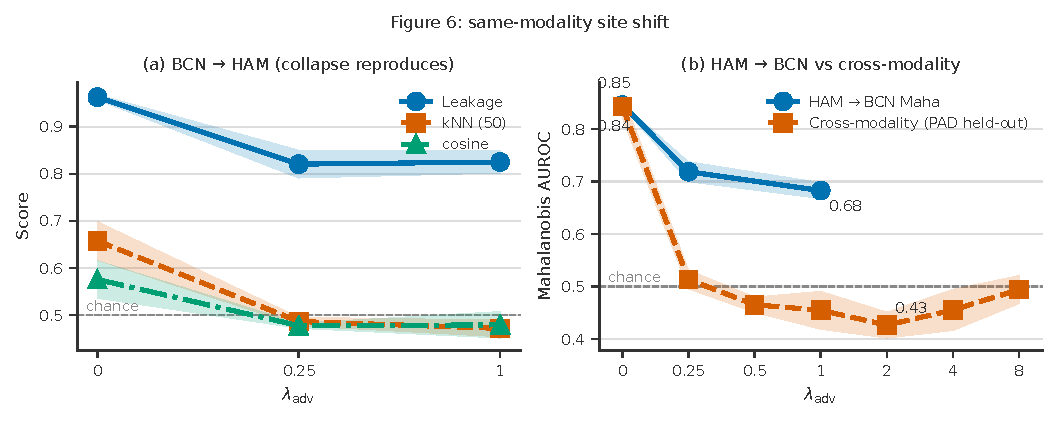
\includegraphics[width=\textwidth]{../../results/paperB/figures/fig6_site_shift.pdf}
\caption{\textbf{A same-modality site shift separates the two claims.} (a) Barcelona to
HAM10000: leakage falls and the detectors with headroom cross chance. (b) With the roles
reversed to restore headroom, Mahalanobis falls from a baseline matching the
cross-modality sweep but stops above chance, while the cross-modality sweep
continues below it.}
\label{fig:site}
\end{figure}

\begin{figure}[t]
\centering
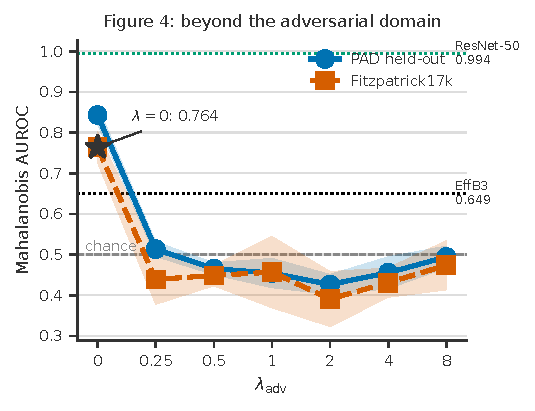
\includegraphics[width=\textwidth]{../../results/paperB/figures/fig4_generalises.pdf}
\caption{\textbf{The collapse is not confined to the adversarial domain.} AUROC against $\lam$
for the held-out PAD partition and for Fitzpatrick17k, which is absent from every
training branch. Horizontal references give the ResNet-50 baseline and the
EfficientNet-B3 control on Fitzpatrick; the controlled comparison is the $\lam = 0$
point of the sweep itself.}
\label{fig:gen}
\end{figure}

\begin{figure}[t]
\centering
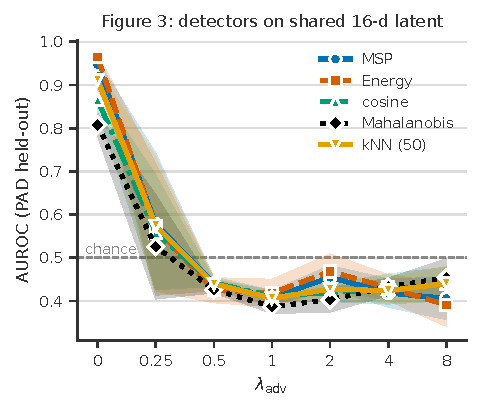
\includegraphics[width=0.72\textwidth]{../../results/paperB/figures/fig3_detectors.pdf}
\caption{\textbf{Every scoring rule moves together.} The five detectors against $\lam$ on the
held-out PAD partition, mean $\pm$ 1 s.d. All five are functions of the same
16-dimensional latent and are therefore not independent evidence;
Figure~\ref{fig:depth} carries the replication on a different representation.}
\label{fig:det}
\end{figure}

\begin{figure}[t]
\centering
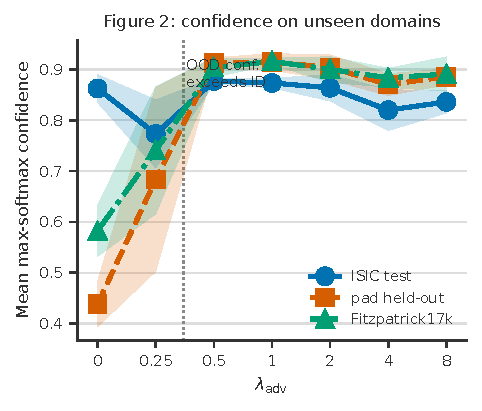
\includegraphics[width=\textwidth]{../../results/paperB/figures/fig2_confidence.pdf}
\caption{\textbf{Confidence on unseen domains overtakes confidence on familiar data.} Mean
maximum-softmax probability against $\lam$ for the ISIC test split, the held-out PAD
partition and Fitzpatrick17k. The crossing occurs by $\lam \approx 0.5$. $\lambda$
spacing is categorical.}
\label{fig:conf}
\end{figure}

\begin{figure}[t]
\centering
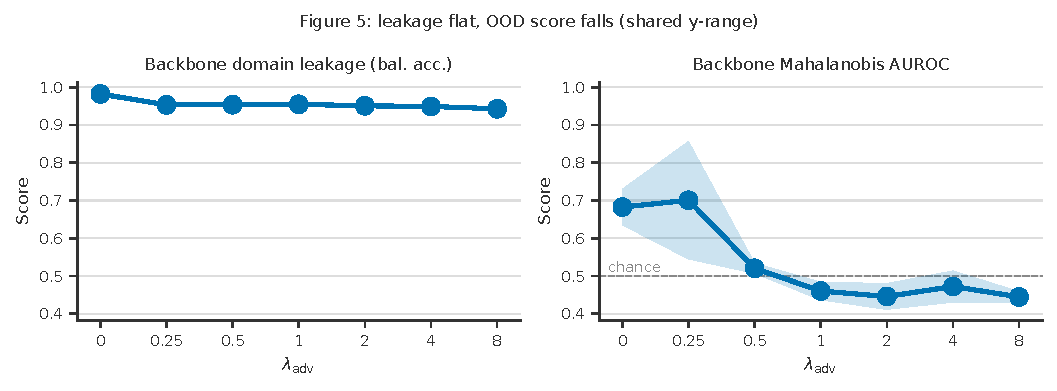
\includegraphics[width=\textwidth]{../../results/paperB/figures/fig5_leakage_no_mediation.pdf}
\caption{\textbf{Leakage does not mediate the collapse.} At the pre-projection backbone the
domain probe stays flat across the sweep while Mahalanobis AUROC falls. Domain
information remains linearly decodable and detection degrades regardless.}
\label{fig:depth}
\end{figure}

\begin{table}[t]
\centering
\small
\caption{Invariance objectives other than gradient reversal, single-encoder backbone,
3 seeds per cell. Leakage is balanced accuracy, floor $0.5$. \textbf{IRM and GroupDRO
use PAD labels} through their environment and group risks; the remaining objectives do
not, so their cross-domain numbers are not comparable and the two regimes are kept in
separate blocks.}
\label{tab:obj}
\begin{tabular}{llcccc}
\toprule
Objective & Weight & Leakage & Maha.\ AUROC & ID bal.\ acc & OOD ECE \\
\midrule
\multicolumn{6}{l}{\emph{No access to PAD labels}}\\
ERM\rlap{$^{\S}$} & ---    & 0.973 & 0.838 & 0.761 & --- \\
CORAL        & 100    & 0.998 & 0.999 & 0.777 & --- \\
MMD          & 1      & 0.967 & 0.813 & 0.779 & --- \\
MMD          & 100    & 0.900 & 0.716 & 0.730 & --- \\
MMD          & 3000   & 0.893 & 0.748 & 0.382 & 0.142 \\
MMD          & 10000  & 0.836 & 0.665 & 0.337 & 0.267 \\
\textbf{GRL} & $\lam = 0.25$ & \textbf{0.763} & \textbf{0.525} & \textbf{0.845\rlap{$^\dagger$}} & --- \\
\midrule
\multicolumn{6}{l}{\emph{Uses PAD labels --- not comparable on cross-domain accuracy}}\\
IRM          & 100    & 0.950 & 0.729 & 0.167 & --- \\
GroupDRO     & 10     & 0.976 & 0.868 & 0.783 & --- \\
\bottomrule
\multicolumn{6}{l}{\footnotesize $^\dagger$ plain accuracy for the GRL row; see Table~\ref{tab:single}.}\\
\multicolumn{6}{l}{\footnotesize $^{\S}$ scored on \texttt{pad\_full} with a uniform optimiser and an ISIC-only loss; the}\\
\multicolumn{6}{l}{\footnotesize \phantom{$^{\S}$} $\lam{=}0$ row of Table~\ref{tab:single} uses \texttt{pad\_heldout}, grouped learning rates and}\\
\multicolumn{6}{l}{\footnotesize \phantom{$^{\S}$} \texttt{ignore\_index}. They are not the same condition. \pending{harmonise or relabel.}}
\end{tabular}
\end{table}

\begin{table}[t]
\centering
\small
\caption{Single-encoder DANN on the same data and splits. ID accuracy is plain accuracy;
leakage is balanced accuracy, floor $0.5$. All five detectors collapse at the smallest
non-zero weight, and four of five fall below chance by $\lam = 4$.}
\label{tab:single}
\begin{tabular}{lccccccccc}
\toprule
$\lam$ & $n$ & Leakage & Maha. & $k$-NN & MSP & cosine & Energy & ID acc & X-dom \\
\midrule
0    & 5 & 0.970 & 0.700 & \textbf{0.944} & 0.868 & 0.884 & \textbf{0.911} & 0.845 & 0.390 \\
0.25 & 3 & \textbf{0.763} & 0.525 & \textbf{0.528} & 0.515 & 0.509 & \textbf{0.507} & 0.845 & 0.333 \\
0.5  & 3 & 0.795 & 0.510 & 0.517 & 0.501 & 0.493 & 0.507 & 0.844 & 0.328 \\
1    & 3 & 0.795 & 0.548 & 0.521 & 0.462 & 0.482 & 0.448 & 0.840 & 0.334 \\
2    & 5 & 0.807 & 0.509 & 0.516 & 0.479 & 0.468 & 0.470 & 0.839 & 0.325 \\
4    & 3 & 0.798 & 0.502 & 0.486 & 0.471 & 0.454 & 0.449 & 0.835 & 0.320 \\
8    & 3 & 0.787 & 0.520 & 0.532 & 0.519 & 0.490 & 0.500 & 0.832 & 0.321 \\
\bottomrule
\end{tabular}
\end{table}

\begin{table}[t]
\centering
\small
\caption{Candidate explanations tested and refuted. Each was a prediction specified
before its test.}
\label{tab:refuted}
\begin{tabular}{p{3.1cm}p{5.2cm}p{6.1cm}}
\toprule
Explanation & Test & Result \\
\midrule
Memorisation of the adversarial images & Hold PAD out of the adversary at patient level & \texttt{pad\_heldout} $0.427$ vs \texttt{pad\_adv} $0.407$; unchanged \\
Class composition & Restrict ID to the six shared classes; reweight ID to the OOD class mix & $0.432$ vs $0.427$ on \texttt{pad\_heldout}; reweighting \emph{strengthens} the inversion to $0.259$ \\
Domain specificity & Evaluate on Fitzpatrick17k, never in $\mathcal{L}_{\mathrm{adv}}$ & $0.391$ at $\lam = 2$ against $0.764$ at $\lam = 0$, same model and data \\
Dimensional collapse & Participation ratio and eigenspectrum across $\lam$ & $4.879 \to 4.500$ while leakage $0.914 \to 0.553$ (same three runs); decoupled \\
Latent compression & Latent variance and distance to centroid across $\lam$ & OOD is already $4.5\times$ tighter at $\lam = 0$; the adversary \emph{decompresses} it \\
Tail asymmetry & Recompute AUROC after truncating the pooled upper tail & $0.412$--$0.424$ versus $0.427$; medians invert \\
\midrule
Synthetic reproduction & Pre-registered toy model with heavy-tailed ID structure, grid fixed before fitting & No inversion ($\lam{=}0$: $0.693$; $\lam{=}2$: $0.786$) \\
\bottomrule
\end{tabular}
\end{table}

\subsection{Confidence, accuracy and calibration on unseen domains}
\label{app:confident}

At $\lam = 0$ the model is appropriately hesitant on unfamiliar data: mean
maximum-softmax confidence is $0.915$ on the ISIC test split and $0.489$ on
\texttt{pad\_heldout}. By $\lam = 0.25$ that gap has closed ($0.913$ versus $0.898$),
and by $\lam = 2$ it has inverted ($0.930$ versus $0.910$).

Cross-domain diagnostic accuracy does not improve at any $\lam$: balanced accuracy
spans $0.249$--$0.291$ against a six-class floor of $0.167$, no setting exceeds the
$0.291$ obtained at $\lam = 0$, and every setting is below the $0.298$ of the
non-adversarial EfficientNet-B3 control. Plain accuracy falls $0.245 \to 0.184$,
beneath the $0.385$ majority-class rate throughout. Macro AUC is roughly preserved
($0.605 \to 0.581$), so discrimination survives while the decision rule does not.

Predictions collapse toward the benign majority class: nevus predictions rise from
$113$ to $374$ of $716$ images, and actinic keratosis recall falls from $0.245$ to
$0.016$ ($49/\nAK \to 3/\nAK$ images, mean over five seeds). Squamous cell carcinoma
moves the same way ($0.088 \to 0.021$, $6/\nSCC \to 1/\nSCC$) but the count is too
small to carry a claim on its own, and melanoma ($n = \nMEL$) supports none.

In this setting out-of-domain ECE is arithmetically close to mean confidence minus
accuracy, which is why the confidence, accuracy and calibration results are not
independent corroboration of each other.

\subsection{Single-encoder replication}
\label{app:single}

Plain single-encoder domain-adversarial training on the same data and splits. Every
detector collapses at $\lam = 0.25$ --- $k$-NN $0.944 \to 0.528$, energy
$0.911 \to 0.507$, cosine $0.884 \to 0.509$, MSP $0.868 \to 0.515$ --- and by
$\lam = 4$ four of the five sit below chance, cosine most clearly at
$0.454 \pm 0.014$. In-distribution accuracy is flat throughout ($0.845 \to 0.832$) and
cross-domain accuracy falls from $0.390$ to a plateau near $0.32$.

\subsection{External replication attempts}
\label{app:external}

\textbf{Camelyon17, three hospitals.} The adversary head never trained:
cross-entropy sat at $\ln 3$ from the first epoch at every $\lam$ while a post-hoc
probe on the same features read $0.94$, despite a gradient graph verified correct
(head cosine $+1.000$, encoder $-1.000$).

\textbf{iWildCam.} The adversary did train --- best-epoch cross-entropy $3.13$ against
$\ln 243 = 5.49$ --- but the encoder never became invariant: the binary
train-versus-OOD site probe moved only from $0.911$ to $0.891$ across
$\lam \in [0, 10]$ against a floor of $0.5$, and no detector collapsed.

\textbf{Camelyon17, two hospitals.} Pre-committed in
\texttt{PRECOMMIT\_CAMELYON2.json} before running. The adversary reached chance
(final cross-entropy $0.692$ against $\ln 2 = 0.693$, from $0.11$ at $\lam = 0$) and
in-distribution accuracy held at $0.995$, but the hospital probe fell only
$0.959 \pm 0.007 \to 0.952 \pm 0.001$, inside its own seed spread, so the leakage gate
failed and the verdict is negative. The exploratory seeds added afterwards do not
reopen it: Mahalanobis on the held-out hospital reads $0.534 \pm 0.050$ at $\lam = 1$
over seeds $42$--$44$, above chance, so the single-seed $0.478$ did not replicate.
These runs appear in Section~\ref{sec:nonmediation} for the non-mediation claim only,
where the five detectors move $0.12$--$0.22$ while the probe moves $0.007$.

\subsection{Same-modality site shift: probe validation and the \texttt{HAM} direction}
\label{app:site}

\textbf{The sites are separable, and not for trivial reasons.} A logistic probe on
frozen ERM features distinguishes \texttt{BCN} from \texttt{HAM} at balanced accuracy
$0.962 \pm 0.007$ against a floor of $0.5$. Masking the dermatoscope vignette reduces
this only to $0.943 \pm 0.005$, so the border is not the signal. Hand-crafted colour
and intensity statistics reach $0.901$ at best --- close to the $0.876$ ceiling the
same features reach on ISIC$\leftrightarrow$PAD, so this pair is no more low-level than
the original contrast --- while sharpness statistics sit at chance ($0.532$). A probe
given only the ground-truth class label reaches $0.668$, reflecting the two sites'
different class distributions; the feature probe is far above that reference.

\textbf{Mahalanobis is uninformative in the \texttt{BCN}-in-distribution direction.} It
reads $0.379$ at $\lam = 0$, already below chance before any adversarial training.
Reweighting the in-distribution set to the out-of-domain class mix raises it to
$0.487$, so most of that baseline inversion is class composition --- \texttt{HAM} is
two-thirds nevus and therefore concentrated near a single well-populated centroid ---
with a residual we attribute to HAM10000's more standardised acquisition and
correspondingly lower feature variance. This is why the reversed direction, which
restores headroom, carries the scope claim in Section~\ref{sec:site}. In that
direction the class-reweighted variant falls from $0.74$ to $0.54$, and Mahalanobis
reads $0.719 \pm 0.019$ at $\lam = 0.25$.

\subsection{A domain monitor is cheap, and semantic novelty is unaffected}

A linear domain head on a frozen ImageNet ResNet-50 that has never seen this data
reaches AUROC $0.998$; on the trained baseline, $0.997$; on the trained EfficientNet-B3
control, $0.991$. Detecting the acquisition domain is easy from almost any
representation, so retaining a monitor is not in itself difficult. What distinguishes
the dual-encoder's context branch is \emph{concentration}: a single principal component
carries $84.5\%$ of its variance and already separates the domains
(AUROC $>0.9999$, two discordant pairs in $11.6$M), against $0.55$--$0.70$ at $k = 1$
for every other representation tested.

The damage is specific to covariate shift. With the domain held constant and diagnostic
classes withheld from training instead, both branches land between $0.6$ and $0.8$ and
the ordering depends on which class is withheld (DF and VASC: lesion $0.648$, context
$0.641$, baseline $0.687$; SCC: lesion $0.806$, context $0.607$, baseline $0.684$). No
near/far structure organises the difference (Pearson $-0.12$ against a
centroid-similarity index). We report this as a null result.

% ------------------------------------------------------------


\end{document}
